\section{Methodology} 
Due to limited time frame this report is limited to the Kalman filter portion of the proposed project. The other aspects will be constructed and available in the future, provided continued operation of the OSNAP program.

Kalman filters are a mathematic way to improve understanding of a time-series linear system. These systems can generally be measured at time steps and have predictive mathematic models, but both of these options have noise or error associated  with them. Kalman filters combine the two and use the error values to adjust how much each is weighted at a given time step. 

The Kalman filter can be parallelized at two levels. It is based on a series of linear algebra equations many of which are independent of each other.  The independence of the different equations suggested that they would be good candidates for task-level parallelism. These equations are based on dense linear algebra equations which have a long history of being efficiently parallelized. This study explored both of these options.

\subsection{Equation Parallelism}

\begin{SCfigure}
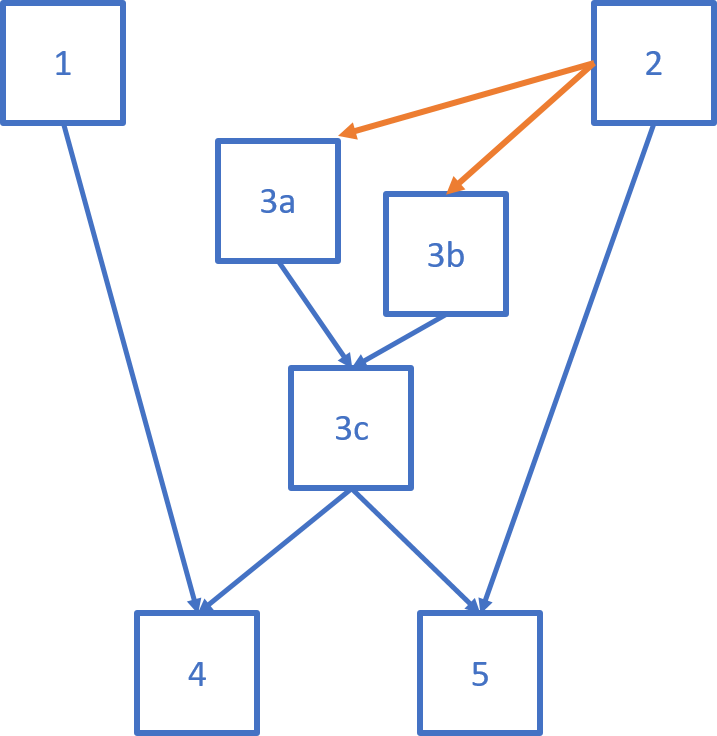
\includegraphics[width=0.4\textwidth]{dag.png}
\label{fig:dag}
\caption{Task graph of Kalman filter, number correspond to the equation in that section. Blue indicates dependencies programmed into the system. Red indicates dependencies erroneously ignored.}
\end{SCfigure}

The Kalman equations (eqs. 1- 5) can be decomposed into seven sections (figure 2) with some dependencies between them. These sections were then sent to separate threads to run concurrently. Several of the equations rely on data computed in previous equations meaning that the computation was divided into two parallel sections. The first of these ran four parallel tasks while the  second ran two and the seventh task had to occur sequentially. Additionally, each time step was serialized since they rely heavily on each other. 


\begin{equation}
\hat{x}_{new} = A\hat{x}
\end{equation}

\begin{equation}
P=APA^T+Q
\end{equation}

\begin{subequations}
\begin{equation}
t_1 = PC^T
\end{equation}
\begin{equation}
t_2 = (CPC^T+R)^{-1}
\end{equation}
\begin{equation}
K = t_1 t_2
\end{equation}
\end{subequations}

\begin{equation}
\hat{x}=\hat{x}_{new} + K(y-C\hat{x}_{new})
\end{equation}

\begin{equation}
P=(I-KC)P
\end{equation}

\subsection{Linear Algebra Parallelism}
Linear algebra operations are highly parallel in that many of the row or elements operations are completely independent of each other, enabling parallel computation. This feature of linear algebra is commonly exploited in scientific computation, graphics and many other domains. It can be applied using hardware accelerators (GPUs, vector instructions, etc), shared memory threads, or distributed processors.

For this report we parallelized the linear algebra functions by applying simple OpenMP pragmas to each function. Primarily this resulted in the parallelization of the outermost for loop of each operation. Some reductions were used as well in the determinant and LU factorization. Generally the parallelization did not include nesting of omp parallel regions, but some resulted because of functions calls within the linear algebra library. For example, the cofactor function includes calls to the LU factorization both of which include omp regions.

For comparison, the library was compiled using the automatic parallelization feature available with Intel's compiler. This feature is intended to automatically exploit parallelism without the assistance of the programmer.

\subsection{Experimental Environment}
 Experiments were run on a single node of the Cerberus cluster. These nodes consist of a quad-core Intel i5 Processor running at 1.3GHz with 16GB of memory and 32KB of L1 cache. Results were recorded using TAU.

For the full Kalman filter experiments we generated 1000 points of noisy projectile motion data. This data is run through the Kalman filter and the process is repeated 1000 times to average out measurement noise. The Kalman filter was tested in four configurations: 1) purely sequential; 2) parallel Kalman with sequential linear algebra; 3) parallel Kalman with OMP linear algebra; and 3) parallel Kalman with Intel parallelized linear algebra.

Similarly, for the linear algebra functions were tested to see how the parallelization affected them independent of the Kalman filter. For these experiments small (6x6) matrices were randomly generated and computations applied to them. Each of the functions was applied to the matrices 100000 times so that the length of computation would be sufficient to compare. 
